\subsection{Diagramme des cas d'utilisation}
    \subsubsection{Cas général}
    \paragraph{}
    \begin{figure}
        \centering
        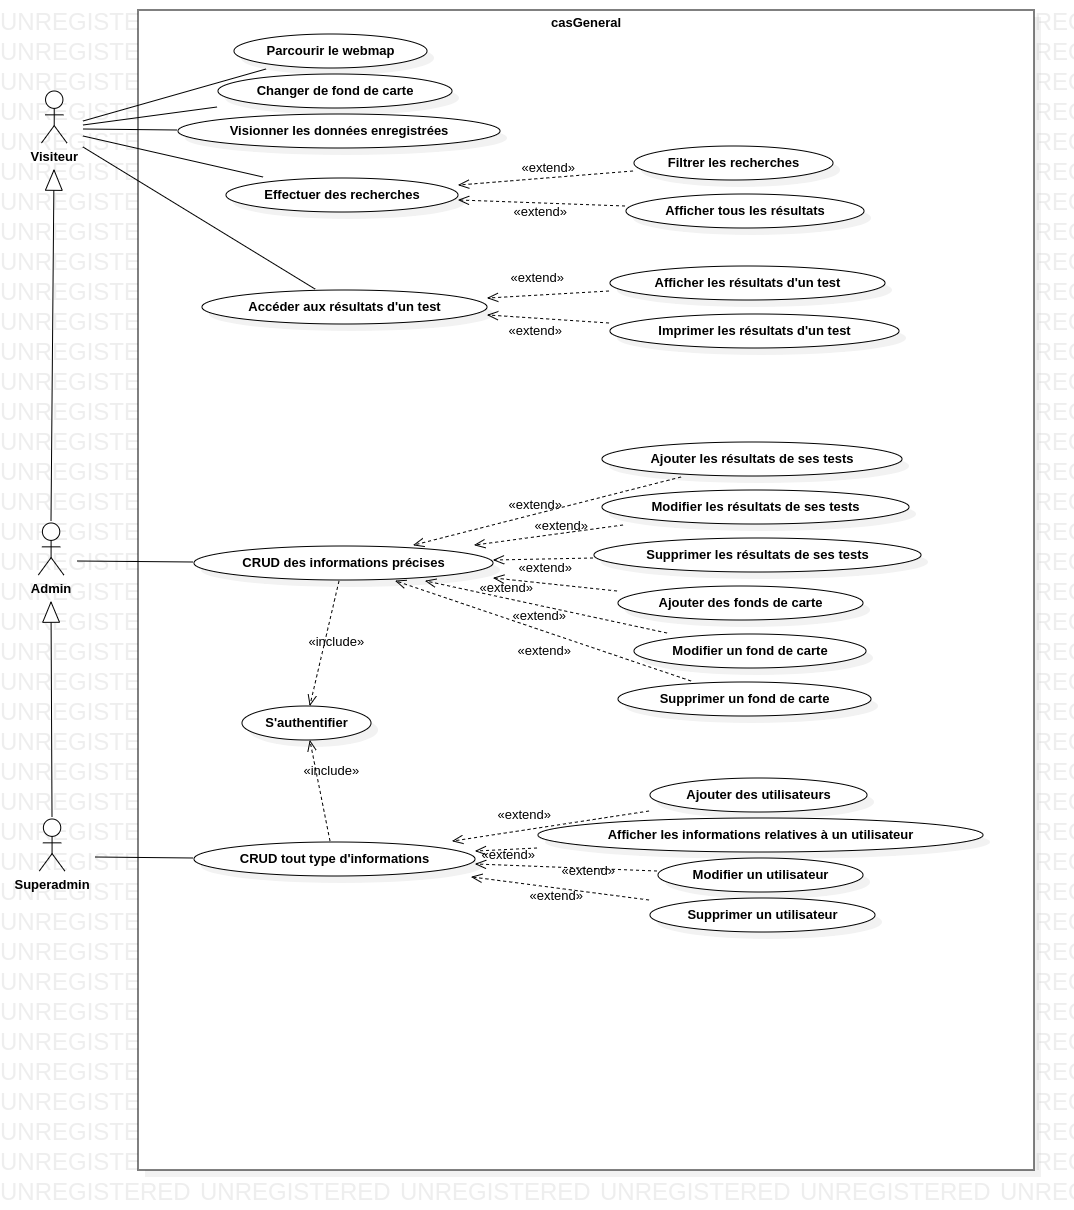
\includegraphics[width=1\textwidth]{casGeneral.png}
        \caption{Diagramme des cas d'utilisation général}
    \end{figure}
    Trois niveaux d'acteurs sont à considérer au sein du système: un visiteur, 
    un administrateur et un super administrateur. La hiérarchisation permet que 
    chaque niveau ait accès aux droits du niveau immédiatement inférieur. 
    De ce fait, un super administrateur sera également un administrateur et 
    un visiteur en plus de son niveau direct. \par 
Pour commencer, le \textbf{visiteur} aura des droits d'accès très restreints: \par 
\begin{itemize}
    \item Parcourir le webmap: Le visiteur pourra voir l'ensemble des informations 
    géotechniques disponibles sur la carte.
    \item Changer de fond de carte: Afin de mieux illustrer le contexte marquant 
    l'intérêt du visiteur, une variété de fonds de carte sera accessible sur le site. 
    Ainsi, l'utilisateur pourra puiser dans le champs de choix qui lui seront proposés.
    \item Visionner les données enregistrées: En cliquant sur un emplacement précis, 
    le visiteur pourra voir les données qui ont été préalablement enregistrées dans la base de données.
    \item Effectuer des recherches: Deux options s'offrent aux utilisateurs: 1) afficher tous les résultats au cours d'une recherche; 2) utiliser 
    des filtres capables de mieux limiter les plages des résultats.
    \item Accéder aux résultats d'un test: Une fois les résultats obtenus, le visiteur 
    pourra soit simplement les afficher, soit les imprimer.
\end{itemize}

\paragraph{}
De son côté, l'\textbf{administrateur} s'occupe de la gestion des informations au sein de la base 
de données. En plus des droits de visiteur, ce type d'utilisateur peut:
\begin{itemize}
    \item Ajouter des informations géotechniques: L'administrateur pourra ajouter des informations 
    dans la BDD, qui seront reflétées sur la carte. 
    \item Modifier les informations qu'il avait préalablement enregistrées: Il ne pourra 
    modifier que les informations qu'il avait lui-même ajoutées.
    \item Supprimer les informations qu'il avait préalablement enregistrées: Tout comme il 
    en est pour la modification, il ne pourra supprimer que les informations qu'il avait lui-même ajoutées.
    \item Ajouter un fond de carte
    \item Supprimer un fond de carte
\end{itemize}

\par 
Évidemment, aucune de ces actions ne saura avoir lieu tant que l'administrateur ne se sera pas authentifié.
\paragraph{}
En dernier lieu, le \textbf{super administrateur} jouera surtout un rôle de gestionnaire en ressources 
humaines. Une fois authentifié, en plus des droits d'accès d'un simple administrateur, 
cet utiliateur pourra:
\begin{itemize}
    \item Ajouter des utilisateurs
    \item Modifier les utilisateurs
    \item Afficher les informations relatives aux différents utilisateurs, pouvant 
    ainsi retracer toutes les actions posées par un utilisateur du système.
    \item Supprimer ou désactiver un utilisateur: La différence se fait remarquer 
    par le fait que le super admin peut supprimer complètement un utilisateur ainsi 
    que toutes les informations y relatives ou simplement désactiver le compte d'un 
    utilisateur sans, pour autant, éliminer ses données.
\end{itemize}
